\chapter{Experiments and Results}

\section{Bouncing Ball Test}
To give credibility to the approach mentioned in \autoref{sec:grid_htm}, a simple test case to test the capabilities of HTM and confirm that they apply on a video is introduced.
\begin{figure}[H]
    \centering
    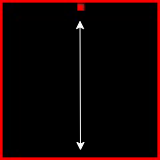
\includegraphics[width=.3\textwidth]{resources/experiments/bouncing_ball/bb_updown1.png}\hfill
    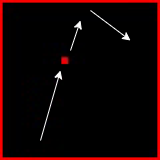
\includegraphics[width=.3\textwidth]{resources/experiments/bouncing_ball/bb_updownside.png}\hfill
    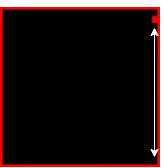
\includegraphics[width=.3\textwidth]{resources/experiments/bouncing_ball/bb_updown2.png}
    \caption{The bouncing ball test, and its three stages}
    \label{fig:bb}
\end{figure}
The video consists of a ball bouncing up and down until an anomaly occurs in the form of a sudden introduction of a horizontal velocity. After a while this horizontal velocity is set back to 0 and the ball is once again bouncing up and down in-place.
\par
\subsection{HTM}
The model used is a standard HTM model, which covers the entire input. This is equivalent to a single cell in a Grid HTM.
\begin{figure}[H]
    \centering
    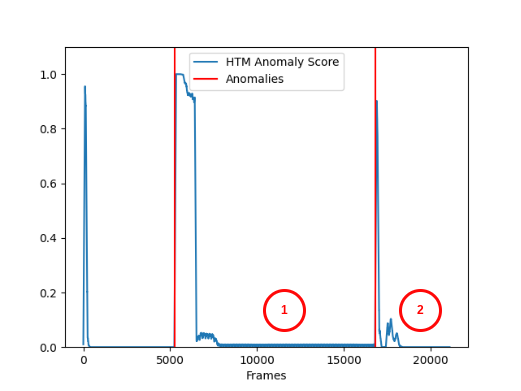
\includegraphics[width=\textwidth]{resources/experiments/bouncing_ball/bb_anoms_bad.png}
    \caption{The 100-point moving average of the anomaly score in the bouncing ball experiment.}
\end{figure}
From the figure it can be observed that the HTM correctly detects anomalies and quickly adapts to them. On the other hand, the result is not perfect due to the minor oscillations close to $(1)$ and the anomaly spikes towards the end close to $(2)$. While the imperfections are not major and can be safely ignored, it is still important to understand their causes and what can be done to improve upon them. \par
\subsubsection{Boosting}
The reason for the oscillations is due to the spatial pooler being dominated by a lucky few columns. The solution is to enable boosting, as explained in \autoref{sec:spatial_pooler}. This also helped with the spikes towards the end, as can be seen in \autoref{fig:bb_boosting}.\par
\begin{figure}[H]
    \centering
    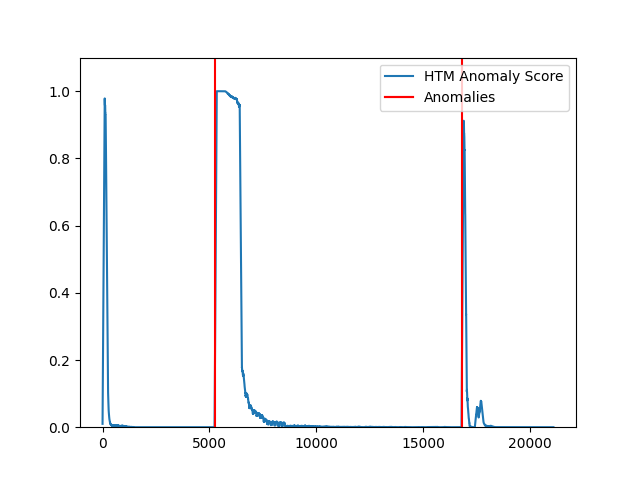
\includegraphics[width=\textwidth]{resources/experiments/bouncing_ball/bb_anoms_boosting.png}
    \caption{Bouncing ball with boosting enabled.}
    \label{fig:bb_boosting}
\end{figure}
\subsubsection{Zero Permanence Decrement}
The reason for the anomaly spikes towards the end is because the spatial pooler has found an optimal representation when the ball is bouncing freely, but when the ball stops and starts bouncing in-place the spatial pooler ends up unlearning the old optimal representation while it learns the new optimal representation. This causes a sudden minor change in the SP output, which the TM reports as anomalous.
\par
The solution is to set the value by which permanence is decreased by to zero, effectively disabling the ability of the spatial pooler to "forget", as can be seen in \autoref{fig:bb_forget}. That being said, the ability to decrement permanence is important in HTM systems, therefore disabling it is not always feasible.
\begin{figure}[H]
    \centering
    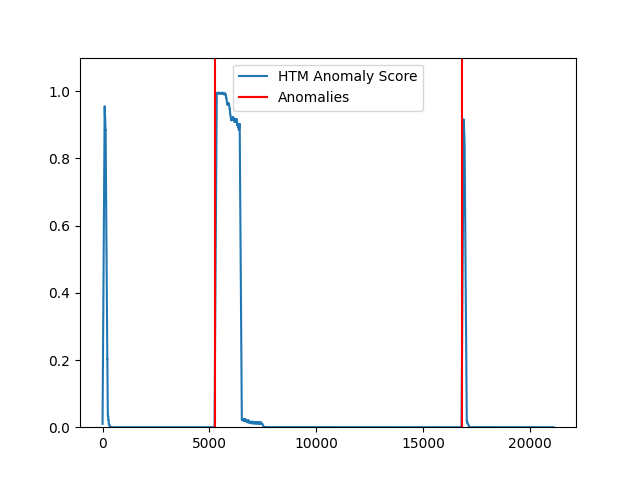
\includegraphics[width=\textwidth]{resources/experiments/bouncing_ball/bb_anoms_unforgetting.png}
    \caption{Bouncing ball without the ability of the SP to "forget".}
    \label{fig:bb_forget}
\end{figure}
\subsubsection{Boosting + Zero Permanence Decrement}
Finally, for the sake of interest, the bouncing ball test was performed with both boosting enabled and with zero permanence decrement. Results can be seen in \autoref{fig:bb_boosting_forget}.
\begin{figure}[H]
    \centering
    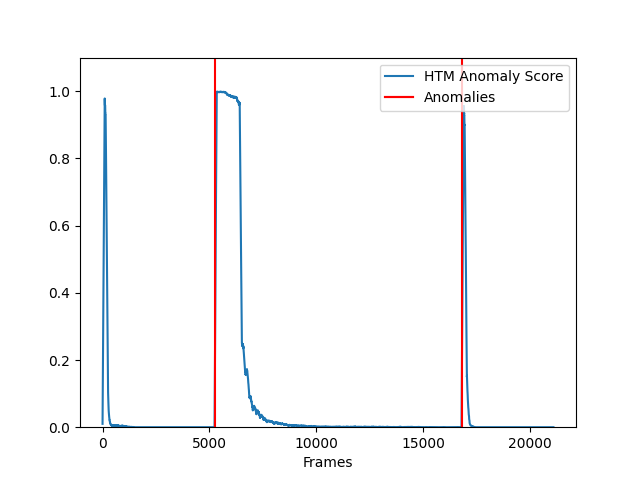
\includegraphics[width=\textwidth]{resources/experiments/bouncing_ball/bb_anoms_unforgetting_boosting.png}
    \caption{Bouncing ball without the ability of the SP to "forget" and with boosting enabled.}
    \label{fig:bb_boosting_forget}
\end{figure}
\subsubsection{Parameters}
Final list of parameters for reproducibility:
\begin{table}[H]
    \centering
    \begin{tabularx}{\linewidth}{@{}llX@{}}
        \toprule
        \textbf{Parameter} & \textbf{Value} & \textbf{Notes}                                      \\
        \midrule
        inputDimensions    & 120, 120       & The shape of the entire frame                       \\
        columnDimensions   & 60, 60         &                                                     \\
        potentialPct       & 0.1            &                                                     \\
        potentialRadius    & 120            &                                                     \\
        localAreaDensity   & 0.02           &                                                     \\
        globalInhibition   & True           & Set to False to enable topology                     \\
        wrapAround         & True           &
        Allows the columns near the edges to "wrap around" and form connections on the other side \\
        synPermActiveInc   & 0.1            &                                                     \\
        synPermInactiveDec & 0              & Set to \textgreater{}0 to enable the SP to "forget" \\
        stimulusThreshold  & 2              &                                                     \\
        seed               & 2              &                                                     \\
        boostStrength      & 0.1            & Set to 0 to disable boosting                        \\
        dutyCyclePeriod    & 250            &                                                     \\
        \bottomrule
    \end{tabularx}

    \caption{SP Parameters}
    \label{tab:bb_sp_params}
\end{table}
\begin{table}[H]
    \centering
    \begin{tabularx}{\linewidth}{@{}llX@{}}
        \toprule
        \textbf{Parameter}        & \textbf{Value} & \textbf{Notes} \\
        \midrule
        columnDimensions          & 60, 60         & Same as the SP \\
        predictedSegmentDecrement & 0.003          &                \\
        permanenceIncrement       & 0.1            &                \\
        permanenceDecrement       & 0.001          &                \\
        minThreshold              & 3              &                \\
        activationThreshold       & 5              &                \\
        cellsPerColumn            & 16             &                \\
        seed                      & 2              &                \\
        \bottomrule
    \end{tabularx}

    \caption{TM Parameters}
    \label{tab:bb_TM_params}
\end{table}
\subsection{Grid HTM}
This is a very simple problem which does not require invariances, making it unsuitable for Grid HTM. Grid HTM would be suitable if there were two or more independent bouncing balls, due to its improved invariance. Still, it is interesting to see how Grid HTM performs compared to normal HTM.
\par
The SP and TM parameters were selected so that they were as close as possible to the normal HTM parameters. The non-zero mean was chosen as the aggregation function.
\begin{figure}[H]
    \centering
    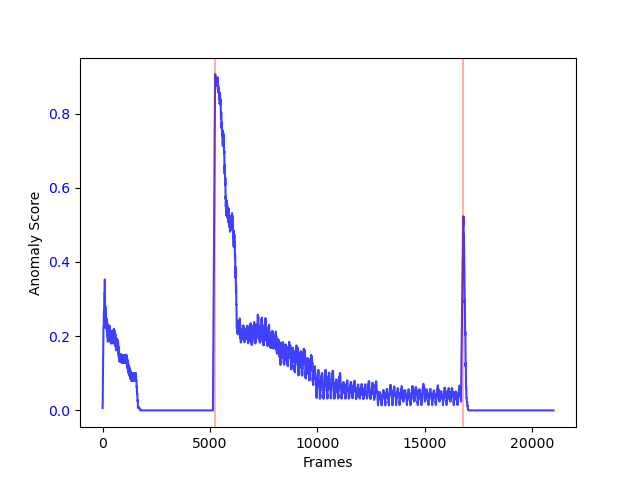
\includegraphics[width=\textwidth]{resources/experiments/bouncing_ball/bb_grid.png}
    \caption{Grid HTM}
\end{figure}
It can be observed that Grid HTM performs worse than the normal HTM, but the result is still acceptable. This is to be expected since this problem is not suited for the Grid HTM, and that the parameters given in \autoref{tab:bb_gridhtm_params}, \autoref{tab:bb_sp_gridhtm_param}, and \autoref{tab:bb_tm_gridhtm_param} are probably not optimal.
% Please add the following required packages to your document preamble:
% \usepackage{booktabs}
\begin{table}[H]
    \centering
    \begin{tabularx}{\linewidth}{@{}XlX@{}}
        \toprule
        \textbf{Parameter} & \textbf{Value} & \textbf{Notes}                                                             \\
        \midrule
        sp\_grid\_size     & 30, 30         & Size of each grid                                                          \\
        tm\_grid\_size     & 15, 15         & Size of each SP grid output.                                               \\
        min\_sparsity      & 1              &                                                                            \\
        sparsity           & A              & Area of the bouncing ball with radius=3                                    \\
        temporal\_size     & 1              & Size of the multistep temporal pattern, 1 means it is effectively disabled \\
        \bottomrule
    \end{tabularx}
    \caption{Grid HTM specific parameters}
    \label{tab:bb_gridhtm_params}
\end{table}
\begin{table}[H]
    \centering
    \begin{tabularx}{\linewidth}{@{}XlX@{}}
        \toprule
        \textbf{Parameter} & \textbf{Value} & \textbf{Notes}                                                  \\
        \midrule
        inputDimensions    & sp\_grid\_size &                                                                 \\
        columnDimensions   & tm\_grid\_size &                                                                 \\
        potentialPct       & 0.5            & Increased in order to compensate for the smaller potential pool \\
        potentialRadius    & 5              &                                                                 \\
        localAreaDensity   & 0.1            &                                                                 \\
        globalInhibition   & True           & Set to False to enable topology                                 \\
        wrapAround         & False          &                                                                 \\
        synPermActiveInc   & 0.1            &                                                                 \\
        synPermInactiveDec & 0.001                                                                            \\
        stimulusThreshold  & 2              &                                                                 \\
        boostStrength      & 0              & Causes instability in empty cells                               \\
        \bottomrule
    \end{tabularx}
    \caption{SP Parameters}
    \label{tab:bb_sp_gridhtm_param}
\end{table}
\begin{table}[H]
    \centering
    \begin{tabularx}{\linewidth}{@{}XlX@{}}
        \toprule
        \textbf{Parameter}        & \textbf{Value} & \textbf{Notes} \\
        \midrule
        columnDimensions          & tm\_grid\_size & Same as the SP \\
        predictedSegmentDecrement & 0.003          &                \\
        permanenceIncrement       & 0.1            &                \\
        permanenceDecrement       & 0.001          &                \\
        minThreshold              & 1              &                \\
        activationThreshold       & 1              &                \\
        cellsPerColumn            & 16             &                \\
        \bottomrule
    \end{tabularx}
    \caption{TM Parameters}
    \label{tab:bb_tm_gridhtm_param}
\end{table}

\section{Surveillance example}
As stated earlier, one of the use cases of Grid HTM is anomaly detection in surveillance. This example will show how Grid HTM could perform.
The video to be used is part of the VIRAT\cite{VIRAT} video dataset, and was selected due to its long duration and stationary camera. The downside is that the video does not contain any anomalies, and also consists of several segments with sudden frame skips in between.
\begin{figure}[H]
    \centering
    \includegraphics[width=0.5\textwidth]{example-image-a}
\end{figure}
As previously mentioned, both binary thresholding and deep learning feature map extraction as encoders have their downsides. Therefore, this thesis proposes to use a combination of both, a segmentation model which can extract classes into their respective SDRs. Meaning that there could be an SDR for cars and an SDR for persons, that are then concatenated before being fed into the system. The segmentation model used is PointRend\cite{pointrend} with a ResNet101\cite{resnet} backbone, pretrained on ImageNet\cite{imagenet}, and implemented using PixelLib\cite{pixellib}.
\begin{figure}[H]
    \centering
    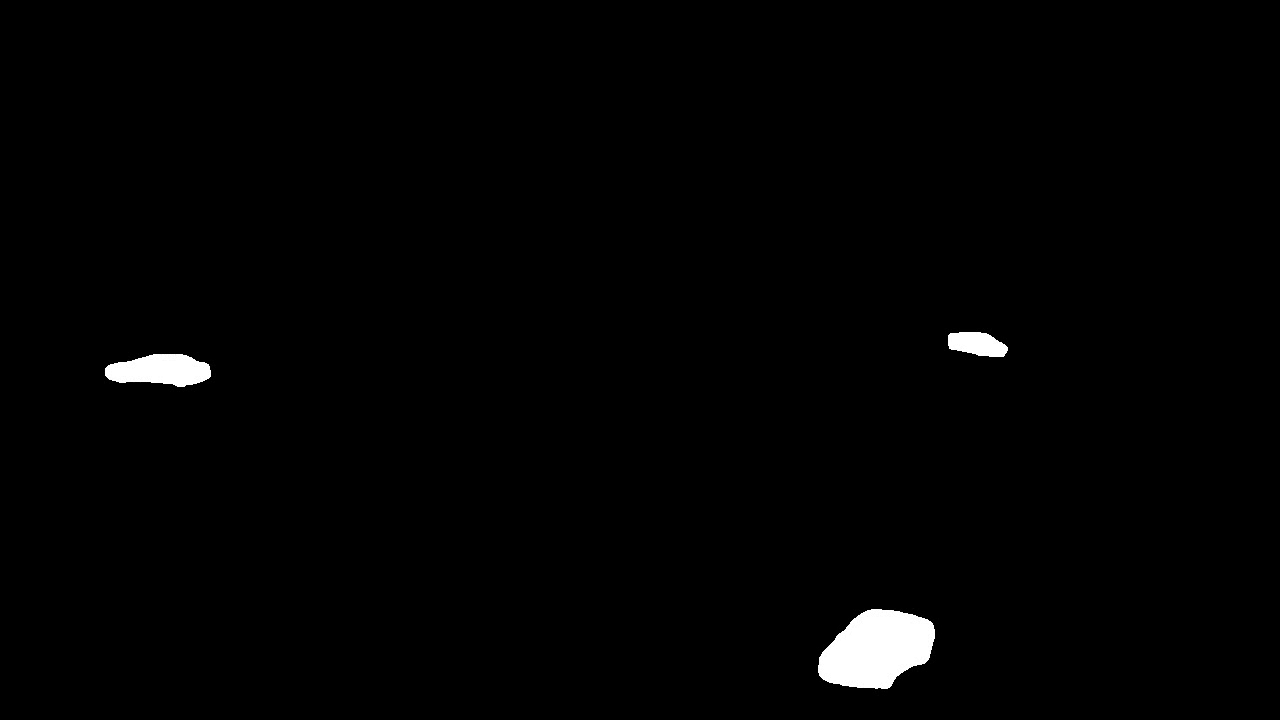
\includegraphics[width=0.45\textwidth]{resources/methodology/car_segmentation.png}
    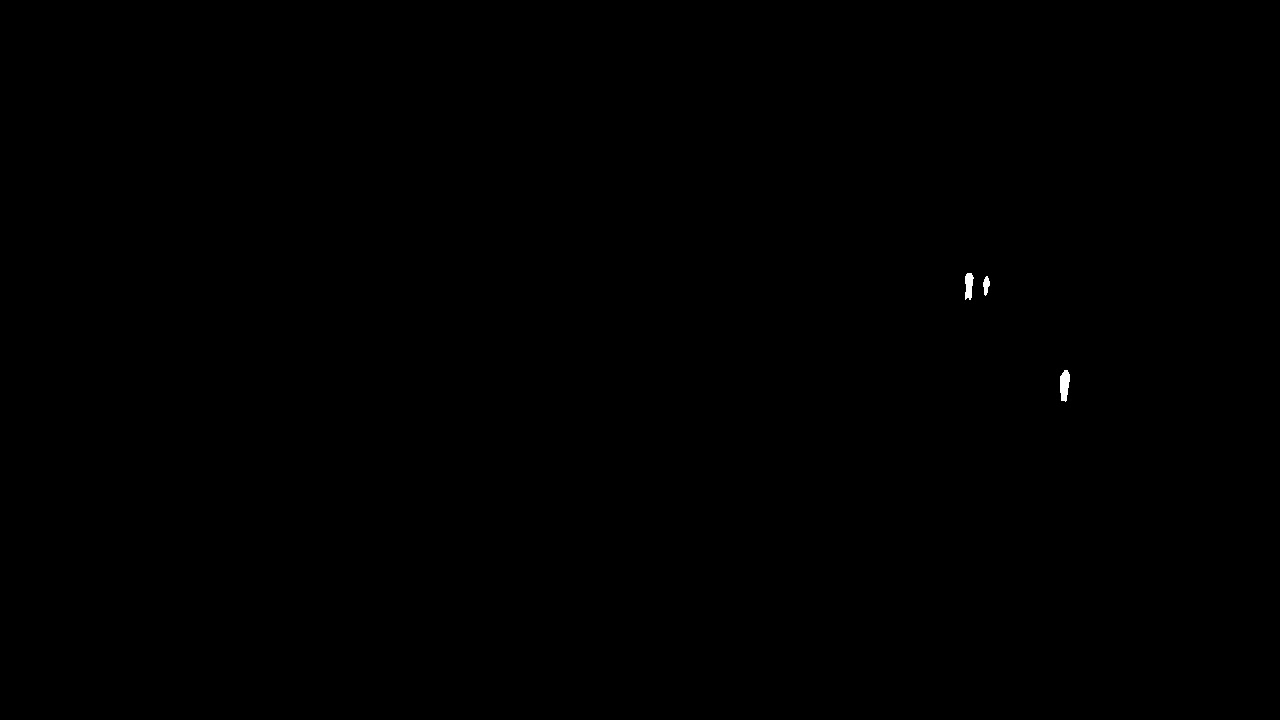
\includegraphics[width=0.45\textwidth]{resources/methodology/person_segmentation.png}
    \caption{Example segmentation of cars and persons.}
\end{figure}
For the sake of simplicity, this experiment will focus only on the segmentation of cars.
\par
While on the topic of segmentation, it is important to mention that the segmentation model is not perfect and that there are cases where objects are misclassified as well as cases where cars repeatedly go above and below the confidence threshold.
\par
\section{Sperm example}
As seen in the surveillance example, it seems the Grid HTM can detect when segments begin and end. This experiment will explore this ability in greater detail.
\subsection{Data}
The dataset used is VISEM \cite{VISEM}, a sperm dataset which consists of videos that are made up of several segments. The sperm cells will be segmented using a rough binary thresholding.
\begin{figure}[H]
    \centering
    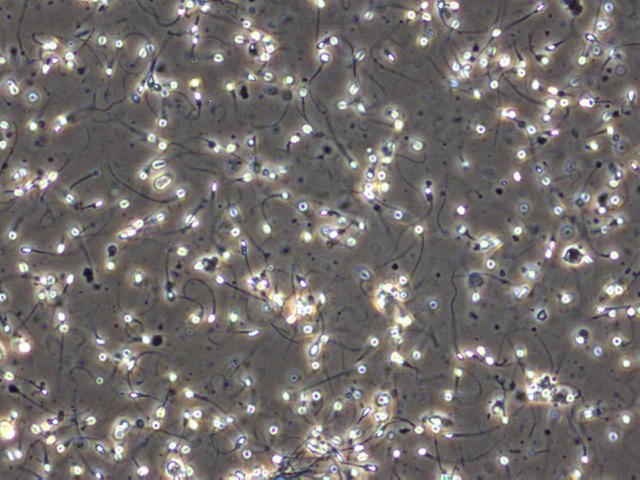
\includegraphics[width=.45\textwidth]{resources/experiments/sperm/sperm_example.png}
    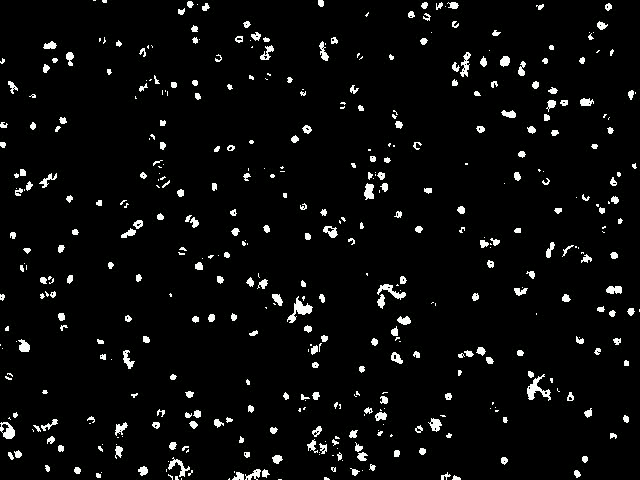
\includegraphics[width=.45\textwidth]{resources/experiments/sperm/sperm_seg_example.png}
    \caption{Example frame from a sperm video and its corresponding segmentation.}
\end{figure}
It is important to note that the data itself is noisy, and that it is not possible for the Grid HTM to learn any meaningful pattern.
\subsection{Benchmark}
To ensure that the HTM does not just react to the sudden change in pixels but does something more, the L1 error will be used as a benchmark to compare against:
\begin{align*}
    E_t=\sum|F_t-F_{t-1}|
\end{align*}
Where $F_t$ denotes a segmented frame at time step $t$.
\subsection{Results}
\begin{figure}[H]
    \centering
    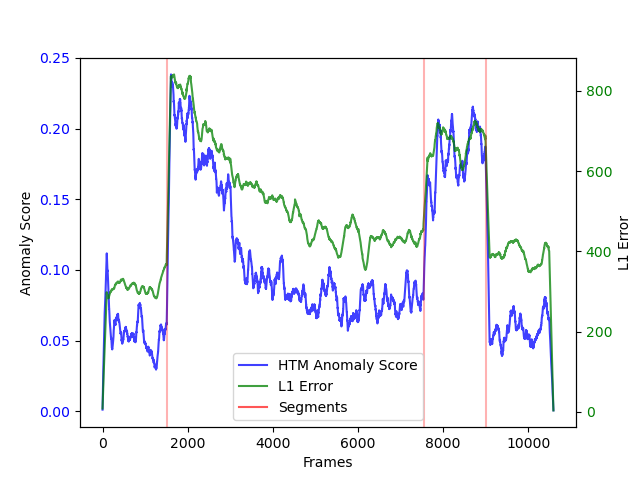
\includegraphics[width=\textwidth]{resources/experiments/sperm/sperm_result1.png}
    \caption{Results.}
    \label{fig:sperm_results1}
\end{figure}
As seen in \autoref{fig:sperm_results1}, the Grid HTM is able to outperform the L1 error benchmark. This can be deduced from the more prominent spikes in the anomaly score, compared to the L1 error. The reason might be that even though the data is very noisy, the Grid HTM is still able to learn something general about the current state. This is most likely a single cell that is standing still, which the Grid HTM anchors itself to and uses it to determine when segments start and end.
\par
That being said, the parameters for the Grid HTM were selected carefully to achieve the results seen in \autoref{fig:sperm_results1}, and are dependent on the contents of the data. Unfortunately, most of the videos in the dataset contain drift (in other words, not stationary), which makes Grid HTM useless. This can be observed in \autoref{fig:sperm_results2}, where both the Grid HTM and the L1 error struggle.
\begin{figure}[H]
    \centering
    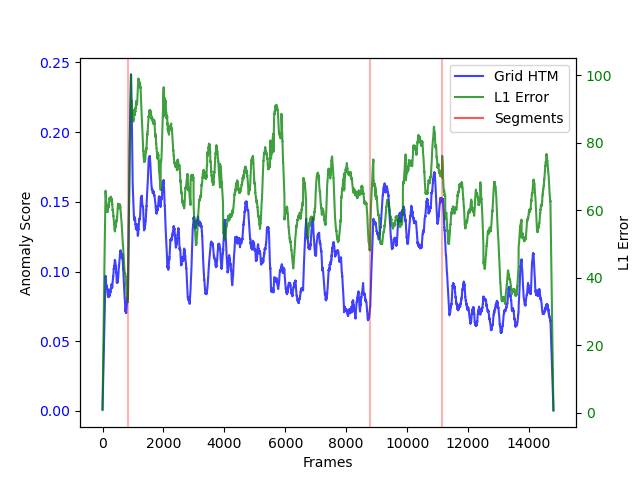
\includegraphics[width=\textwidth]{resources/experiments/sperm/sperm_result2.png}
    \caption{Results.}
    \label{fig:sperm_results2}
\end{figure}